% =================================================================================================
% File:			dia_seq_server.tex
% Description:	Definisce la sezione relativa al capitolo relativo ai diagrammi di sequenza tra i componenti del client
% Created:		2015-05-22
% Author:		Faccin Nicola
% Email:		faccin.nicola@mashup-unipd.it
% =================================================================================================
% Modification History:
% Version		Modifier Date		Change											Author
% 0.0.1 		2015-05-22 			creato scheletro doc							Nicola Faccin
% =================================================================================================
% 0.0.2			2015-05-23			iniziata stesura sezioni						Tesser Paolo
% =================================================================================================
% 0.0.3			2015-05-24			iniziata descrizione oggetti					Tesser Paolo
% =================================================================================================
%

% CONTENUTO DEL CAPITOLO

\subsection{Client} % (fold)
\label{ssub:diagrammi_di_sequenza_client}
Quasi tutte le operazioni offerte dall'applicazione comportano lo stesso tipo di interazione tra le classi presenti nella componente client. Ne sono quindi state descritte alcune ritenute tra le più significative. \newline
Questi diagrammi riguardano solo la parte appunto del client. La comunicazione quindi con il server e le operazioni che esso esegue per ritornare dei valori al client viene mostrata nella sezione \ref{ssub:diagrammi_di_sequenza_server}.

	\subsubsection{Login} % (fold)
	\label{ssub:login}
	Il seguente diagramma di sequenza descrive le collaborazioni tra gli oggetti del front-end dell'applicazione durante l'operazione di autenticazione. \newline


\begin{figure}[htbp]
	\centering
	\centerline{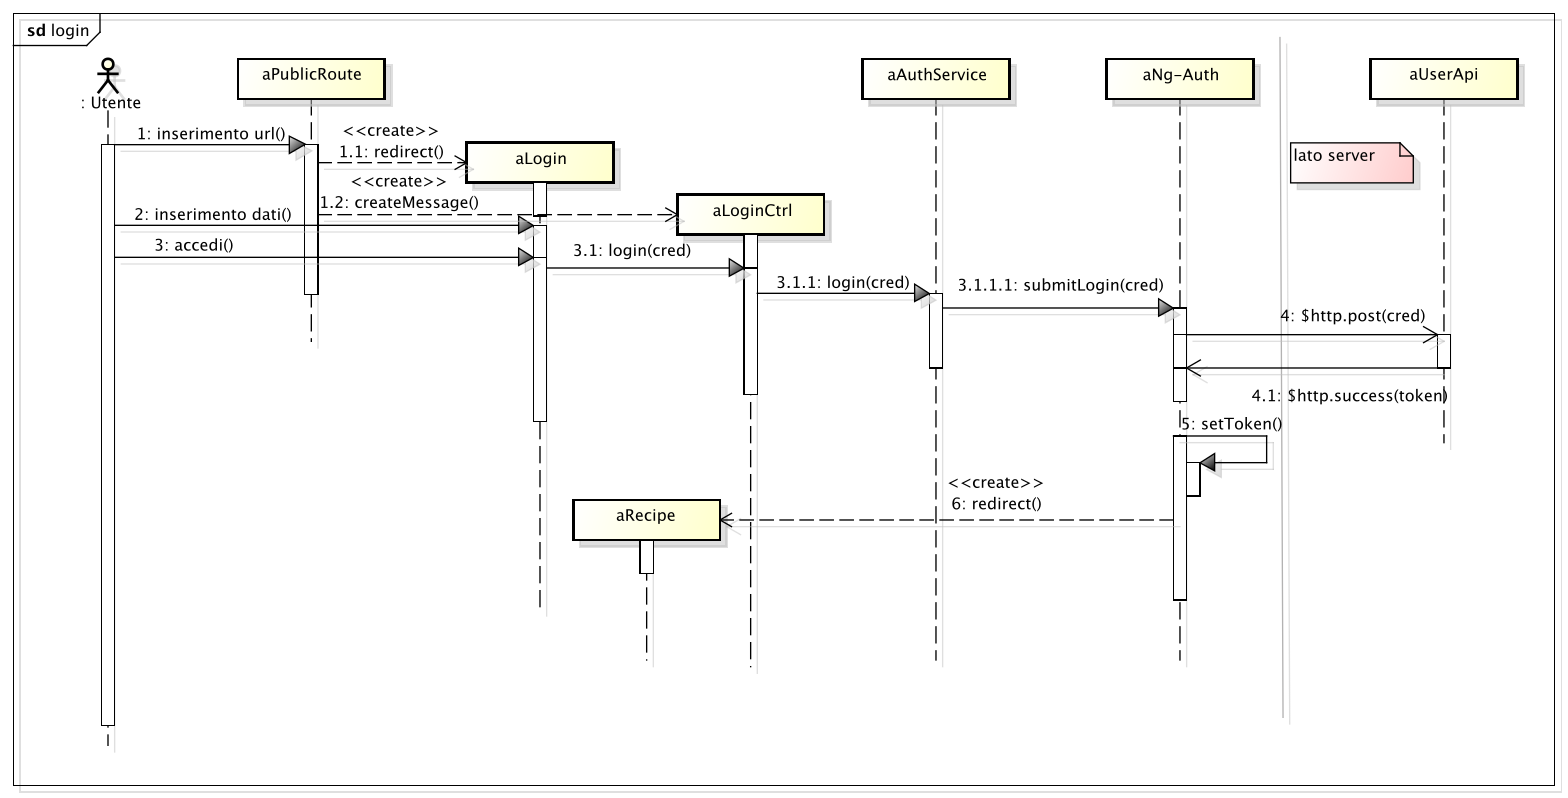
\includegraphics[scale=1.03]{./images/sequence_diagram/client_login.pdf}}
	\caption{Diagramma di sequenza - Login lato client}
\end{figure}



	Il diagramma descrive le interazioni tra gli oggetti che compongono il front-end quando un utente vuole effettuare il login nell'applicazione.
	\begin{itemize}
		\item \textbf{Utente non autenticato}: l'oggetto Utente non autenticato individua un qualsiasi attore che vuole effettuare l'accesso al sistema. L'utente inserisce i propri dati e preme il bottone \'Login\';
		\item \textbf{aPublicRoute}: l'oggetto aPublicRoute re-indirizza l'utente alla corretta pagina, dalla quale potrà effettuare l'accesso;
		\item \textbf{aLogin (login.html)}: l'oggetto aLogin è la vera pagina che permette l'autenticazione dell'utente. Qui verranno inserite le credenziali per accedere e sarà presente il pulsante che una volta premuto invocherà il metodo \textbf{login(cred)};
		\item \textbf{aLoginCtrl}: l'oggetto aLoginCtrl è il controller che si occupa di gestire le funzioni disponibili in \textbf{aLogin}, in particolare di \textbf{login(cred)}. Questo metodo invoca ulteriormente il metodo \textbf{login(cred)} dell'oggetto \textbf{aAuthService} passandogli come parametro un oggetto JSON contenete le credenziali recuperate dal form di inserimento;
		\item \textbf{aAuthService}: l'oggetto aAuthService chiama il metodo \textbf{submitLogin(cred)} del servizio aNg-Auth
		\item \textbf{aNg-Auth}: l'oggetto aNg-Auth rappresenta un modulo esterno, iniettato come servizio tramite Dependency Injection, che gestisce le principali azioni di un utente per quando riguarda autenticazione, registrazione, cambio dati personali, etc. In questo caso viene utilizzato per autenticare un utente al sistema. Una volta ricevuta risposta dal server, viene immagazzinato un access token riguardante la sessione in corso. Attraverso quel token si potranno recuperare tutte le informazioni dell'utente ed effettuare determinate azioni previste dall'applicativo;
		\item \textbf{aRecipe (recipe.html)}: l'oggetto aRecipe è la pagina nella quale l'utente che ha inserito le credenziali corrette viene re-indirizzato.
		\item \textbf{aUserApi}: l'oggetto aUserApi viene usato in questo diagramma per rappresentare il Server, che riceve la chiamata REST dal client e restituisce in risposta i dati richiesti.
	\end{itemize}
	% subsubsection login (end)

	\subsubsection{Visualizzazione delle Recipe} % (fold)
	\label{ssub:visualizzazione_delle_recipe}
	Il seguente diagramma di sequenza descrive le collaborazioni tra gli oggetti del front-end dell'applicazione durante la visualizzazione delle Recipe. \newline

\begin{figure}[htbp]
	\centering
	\centerline{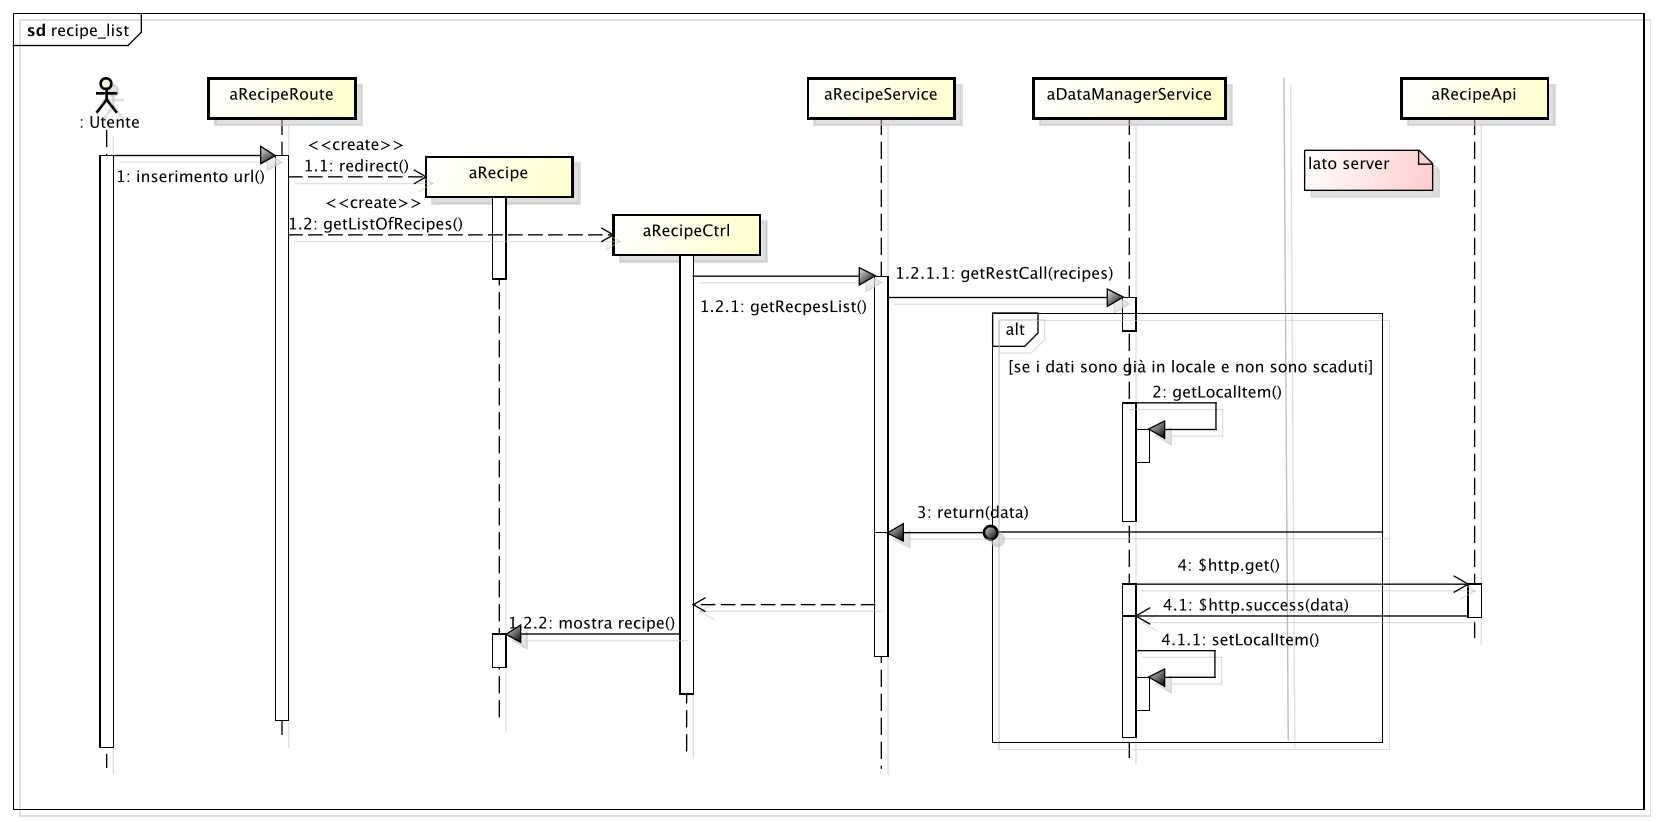
\includegraphics[scale=1.03]{./images/sequence_diagram/client_view_recipe.pdf}}
	\caption{Package - client::controller}
\end{figure}

	

	Il diagramma descrive le interazioni tra gli oggetti che compongono il front-end quando un utente vuole visualizzare la lista delle Recipe presenti nel sistema.
	\begin{itemize}
		\item \textbf{Utente autenticato}: l'oggetto Utente individua un utente che ha effettuato l'accesso al sistema;
		\item \textbf{aRecipeRoute}: l'oggetto aRecipeRoute re-indirizza l'utente alla corretta pagina, dalla quale potrà visualizzare la lista di tutte le recipe;
		\item \textbf{aRecipe (recipe.html)}: l'oggetto aRecipe è la vera pagina che permette la visualizzazione di tutte le recipe presenti nel sistema. La schermata viene riempita grazie all'invocazione in automatico del metodo \textbf{getListOfRecipes()};
		\item \textbf{aRecipeCtrl}: l'oggetto aRecipeCtrl è il controller che si occupa di gestire le funzioni disponibili in \textbf{aRecipe}, in particolare del metodo \textbf{getListOfRecipes()} che chiama ulteriormente il metodo \textbf{getRecipesList()} dell'oggetto \textbf{aRecipeService};
		\item \textbf{aRecipeService}: l'oggetto aRecipeService attraverso la chiamata al metodo \textbf{getRestCall('recipes')} del servizio \textbf{aDataManagerService} fa ritornare una promise all'oggetto \textbf{aRecipeCtrl} che verrà risolta quando la chiamata sarà eseguita correttamente;
		\item \textbf{aDataManagerService}: l'oggetto aDataManagerService riceve le direttive da impostare per effettuare la chiamata al server. Prima di effettuare la chiamata vera e propria però controlla se i dati richiesti non siano già presenti nel localStorage o che non siano troppo vecchi, attraverso l'invocazione del metodo \textbf{getLocalItem(key)} dove il parametro key rappresenta l'indirizzo della chiamata http, che viene usato come chiave per salvare i dati in locale. Se i dati sono presenti gli restituisce incapsulandoli in una promise che verrà risolta immediatamente, altrimenti effettua la chiamata vera e proprio invocando il metodo \textbf{httpGetRequest} dell'oggetto stesso. Una volta ricevuti i dati, il metodo \textbf{setLocalItem(key, value)} provvederà a salvarli in locale;

		\item \textbf{aRecipeApi}: l'oggetto aRecipeApi viene usato in questo diagramma per rappresentare il Server, che riceve la chiamata REST dal client e restituisce in risposta i dati richiesti.
	\end{itemize}
	% subsubsection visualizzazione_delle_recipe (end)

	\subsubsection{Generazione dei grafici} % (fold)
	\label{sub:generazione_dei_grafici}
	Il seguente diagramma di sequenza descrive le collaborazioni tra gli oggetti del front-end dell'applicazione durante la generazione di grafici da una metrica. \newline

\begin{figure}[htbp]
	\centering
	\centerline{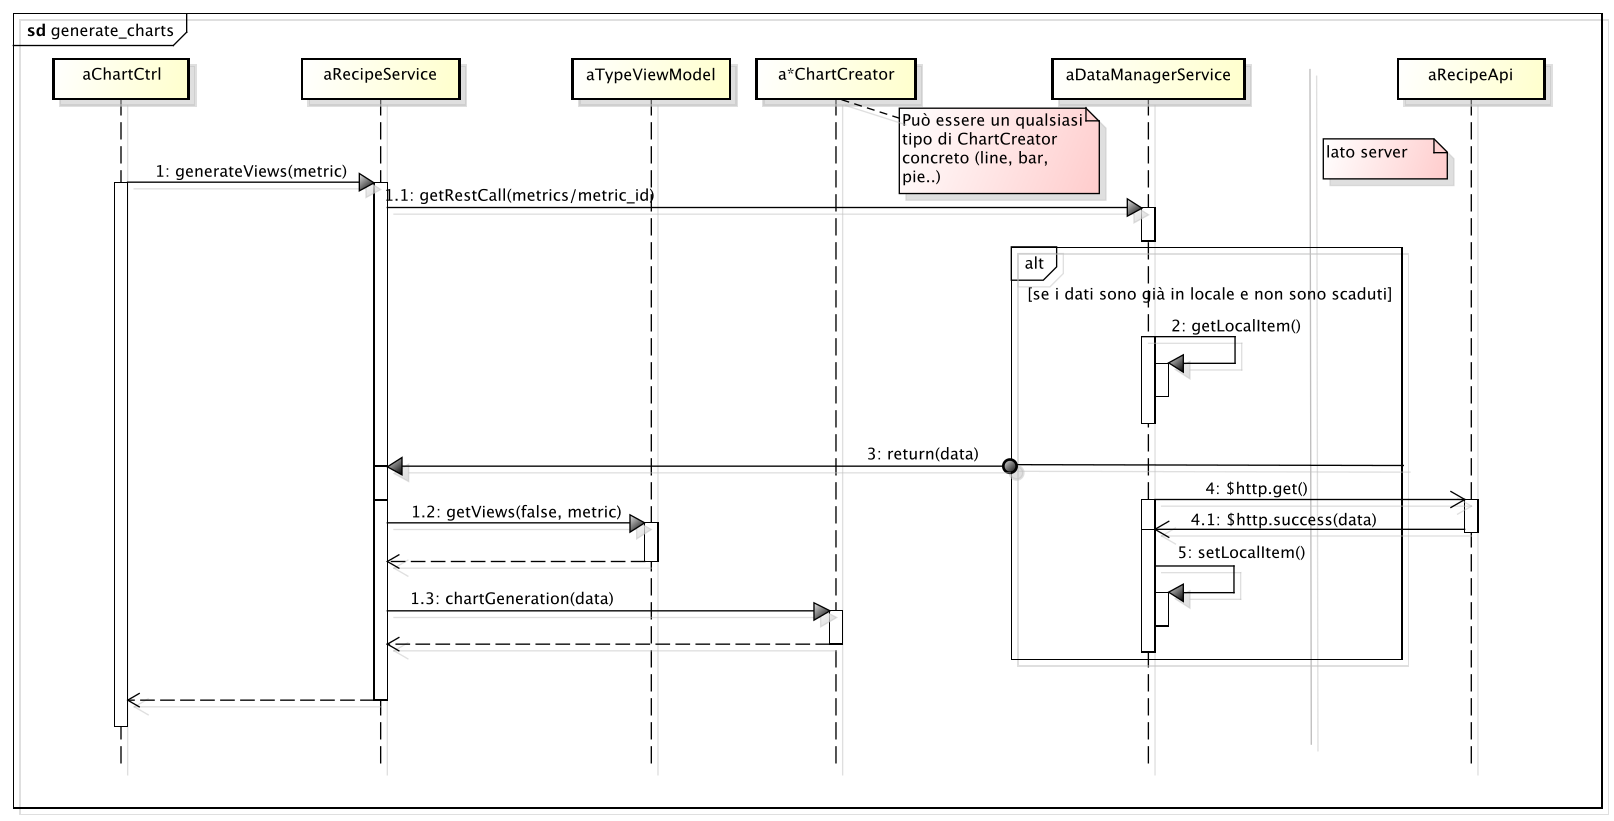
\includegraphics[scale=1.03]{./images/sequence_diagram/client_chart_generation.pdf}}
	\caption{Package - client::controller}
\end{figure}

	

	Il diagramma descrive le interazioni tra gli oggetti che compongono il front-end quando devono essere generati i grafici relativi ad una specipica metrica.
	\begin{itemize}
		\item \textbf{aChartCtrl}: l'oggetto aChartCtrl è il controller che si occupa di gestire le funzioni di visualizzazione di grafici, e che ne richiede la generazione quando è necessario;
		\item \textbf{aRecipeService}: l'oggetto aRecipeService attraverso la chiamata al metodo \textbf{getRestCall('metrics/metric\_id')} del servizio \textbf{aDataManagerService} fa ritornare una promise all'oggetto \textbf{aRecipeCtrl} che verrà risolta quando la chiamata sarà eseguita correttamente. Successivamente tramite la chiamata al metodo \textbf{getViews('false', metric)} otterrà dall'oggetto \textbf{aViewTypeModel} quali tipi di grafici dovranno essere generati. Ottenuta questa informazione attraverso la chiamata \textbf{chartGeneration(data)} avente come parametro le informazioni della metrica e quelle ottenute dall'oggetto \textbf{aViewTypeModel} otterrà i grafici generati, che poi potrà restituire all'oggetto \textbf{aChartCtrl};
		\item \textbf{aDataManagerService}: l'oggetto aDataManagerService riceve le direttive da impostare per effettuare la chiamata al server. Prima di effettuare la chiamata vera e propria però controlla se i dati richiesti non siano già presenti nel localStorage o che non siano troppo vecchi, attraverso l'invocazione del metodo \textbf{getLocalItem(key)} dove il parametro key rappresenta l'indirizzo della chiamata http, che viene usato come chiave per salvare i dati in locale. Se i dati sono presenti gli restituisce incapsulandoli in una promise che verrà risolta immediatamente, altrimenti effettua la chiamata vera e proprio invocando il metodo \textbf{httpGetRequest} dell'oggetto stesso. Una volta ricevuti i dati, il metodo \textbf{setLocalItem(key, value)} provvederà a salvarli in locale;
		\item \textbf{aTypeViewModel}: l'oggetto aTypeViewModel restituisce all'oggetto \textbf{aRecipeService} i tipi di grafici che devono essere generati a partire dalla metrica che riceve quando viene chiamato il suo metodo \textbf{getViews('false', metric)};
		\item \textbf{a*ChartCreator}: l'oggetto a*ChartCreator è in realtà un'istanza di una delle classi figlie di ChartCreator.Questo restituisce i grafici generati a partire dai dati che riceve nella chiamata al suo metodo \textbf{chartGeneration(data)} effettuata da \textbf{aRecipeService};
		\item \textbf{aRecipeApi}: l'oggetto aRecipeApi viene usato in questo diagramma per rappresentare il Server, che riceve la chiamata REST dal client e restituisce in risposta i dati richiesti.
	\end{itemize}
		% subsection visualizzazione_dei_grafici (end)
% section diagrammi_di_sequenza_client (end)